\documentclass[a4paper,12pt]{article}
\usepackage[toc,page]{appendix}
\usepackage{listings}
\usepackage{hyperref}
\usepackage{graphicx}
\usepackage[skip=0pt]{caption}
\usepackage{multicol}
\usepackage{float}
\usepackage[margin=1in]{geometry}
\usepackage{tabularx}

\begin{document}

\renewcommand{\thelstlisting}{\thesection-\arabic{lstlisting}}
\renewcommand{\thefigure}{\arabic{section}-\arabic{figure}}
\setlength{\floatsep}{0pt plus 2pt minus 2pt}
%\setlength{\intextsep}{0pt plus 2pt minus 2pt}
%\setlength{\textfloatsep}{0pt plus 2pt minus 2pt}

\title{Introduction to Digital Libraries Assignment \#2}
\date{March 04, 2015}
\author{James Tate II}
\maketitle

\section{Introduction}
%This assignment required downloading \emph{tweets} from \emph{Twitter} using its API and processing the HTTP URIs
The first part of this assignment required using several tools to create
WARC\footnote{http://www.digitalpreservation.gov/formats/fdd/fdd000236.shtml} files from approximately 100
of the final URIs identified in assignment one. A sample of the WARC files were \emph{replayed} in two WARC
replay tools, to examine their archiving accuracy compared to a web browser's rendering of the original URI
representation. The tools performed wildly differently on different URIs, and the two replay tools even
had different outputs from the same WARC files.

The second part of this assignment required me to setup SOLR\footnote{http://lucene.apache.org/solr/} and
index some of the downloaded WARC files. SOLR is an open-source indexing and search tool --- sample
queries and results are given later in this document.

\section{Methodology}
%info about the different methods used
This assignment required four tools be used to attempt to create WARC files for 100 URIs. Unfortunately, one
of the tools, WAIL\footnote{http://matkelly.com/wail/}, could not be coerced into properly creating WARC
files for the URIs it was given. In short, I ran out of time and patience while trying to make Heritrix, the
web crawler part of WAIL, download only the given URI and not hundreds of other pages. The other three tools
were WARCreate, wget and WebRecorder.io. Before any of these tools could be used, I had to select 
100 URIs to process.

\subsection{URIs}
To select the URIs, I first ordered all the unique final URIs from the first assignment by descending frequency.
Then, from the 200 most frequently-occurring URIs, I excluded the URIs that were not text/html webpages,
appeared to be spam or did not render correctly in a web browser. This left me with 144 URIs of the original
200. Then, I started using the three tools to create WARC files from the URIs until I had successfully created a
WARC file using at least one method from a few more than 100 URIs.

\subsection{wget}
The first, and most simple, tool for creating WARC files from URIs was the *nix utility, wget. In a bash script,
I called the below wget command once for each URI. This command downloads the given URI and supporting pages,
then combines that content into a WARC file. This invocation ignores robots.txt and stores the downloaded web
content in the garbage directory to keep it away from the output WARC files.
\begin{lstlisting}[basicstyle=\ttfamily,caption={Downloading Tweets}]
    wget --warc-file="$2/$id" -p -l 1 -H -e robots=off \
    -P "garbage/" "$uri" > "$2/${id}.wget.output" 2>&1"
\end{lstlisting}
Output from this command is saved in the \emph{X}.wget.output files where \emph{X} is the id of the URI. The
generated WARC files are compressed with gzip and saved in \emph{X}.warc.gz files. wget was by far the easiest
tool used to create WARC files, mostly due to its usability in simple bash scripts.

\subsection{WARCreate}
WARCreate is a Google Chrome extension that allows the user to create a WARC file of the currently visible
webpage. Using WARCreate was troublesome and produced interesting results (see Section 3.2). Most frustratingly,
Chrome had to be restarted frequently to counteract the continual slowdowns of WARCreate. By design, I had to
manually click the ``Generate WARC'' button on each of over 100 webpages after navigating to the URI in
the web browser. I had to wait for the extension to give
me a WARC file to save after clicking the button.
Sometimes, after waiting 30 or more seconds, I would give up and move on to the next URI without ever getting
a WARC.

\subsection{WebRecorder.io}
WebRecorder.io is a website available at \url{http://webrecorder.io}. It allows the user to, at no cost,
``record'' webpages and download the resulting WARC files. It also allows users to upload WARC files created
by it and other tools to ``replay'' them in the web browser. Both of these functions were used in this
assignment. See the Section 3.2 for details on playback using WebRecorder.io.

Using WebRecorder.io required me to paste the URI into a text field on the website, and click the ``Record''
button. Then, after the page rendered for a couple seconds, I could immediately download a WARC file.
Although a few pages did not render correctly on WebRecorder.io, which required those URIs to be skipped,
WebRecorder.io was a relatively pain-free tool to use. WARC files downloaded from WebRecorder.io were also
compressed with gzip.

\subsection{SOLR}
Apache SOLR was the search platform used to test indexing and searching of the generated WARC files. It was
simple to run on Linux by downloading the binary from the Apache website, along with the Maven binary also
from Apache. The commands below were used to run SOLR from the pre-compiled binaries.
\begin{lstlisting}[basicstyle=\ttfamily,caption={Downloading Tweets}]
export PATH=$PATH:/home/jtate/src/apache-maven-3.2.5/bin/
mvn jetty:run-exploded -Djetty.port=10770
java -jar warc-indexer-2.0.1-20150116.110435-2-jar-with-dependencies.jar \
-s http://localhost:10770/discovery -t ../../cs751/warc/wget/*.warc.gz
\end{lstlisting}
The last command (split across two) lines, was used to add all WARC files generated by wget to SOLR's
search index/database. The web interface to SOLR allowed queries to be entered and would display the
responses in JSON format. See section 3.3 for SOLR results.

\section{Results}
This section describes the observed performance of WARC creation and playback, as well as searching using
SOLR.

\subsection{WARC Files}
The WARC files generated by the three tools each had different properties. Some quantitative properties of
the WARC files generated by the three tools are shown in the table below.
\begin{figure}[H]
\centering
\begin{tabular}{ | c | c | c | c | }
\hline
WARC Tool                   & wget      & WARCreate & WebRecorder.io    \\ \hline
Number of WARC Files        & 166       & 106       & 113               \\ \hline
Average WARC Size           & 6.23MB    & 8.27MB    & 2.41MB            \\ \hline
Average Number of Requests  & 103.3     & 1048      & 86.73             \\ \hline
Average Number of Responses & 103.2     & 331.1     & 82.74             \\ \hline
\end{tabular}
\end{figure}
The table lists the number of WARC files 

\subsection{Playback}


\subsection{SOLR Queries}



%\begin{figure}[H]
%    \centering
%    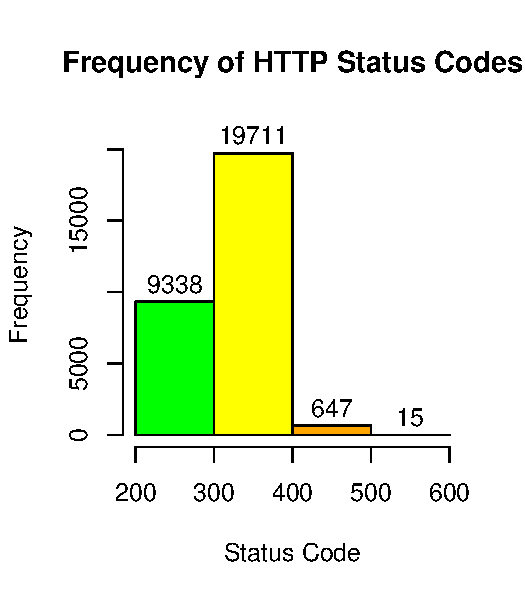
\includegraphics{stats/http_status_codes.pdf}
%    \caption{Frequency of HTTP status codes in histogram by sequential category.}
%\end{figure}


\clearpage
\begin{appendices}

\section{Streaming API Filter Keywords}

\end{appendices}




\clearpage
\begin{thebibliography}{9}
%\bibitem{rfc2616}
%    R. Fielding, et. al.,
%    \emph{Hypertext Transfer Protocol -- HTTP/1.1}.
%    \url{https://www.ietf.org/rfc/rfc2616.txt}
%    June 1999.

\end{thebibliography}

\end{document}
